\documentclass[tikz,border=3.14mm]{standalone}
\usetikzlibrary{patterns}

\begin{document}
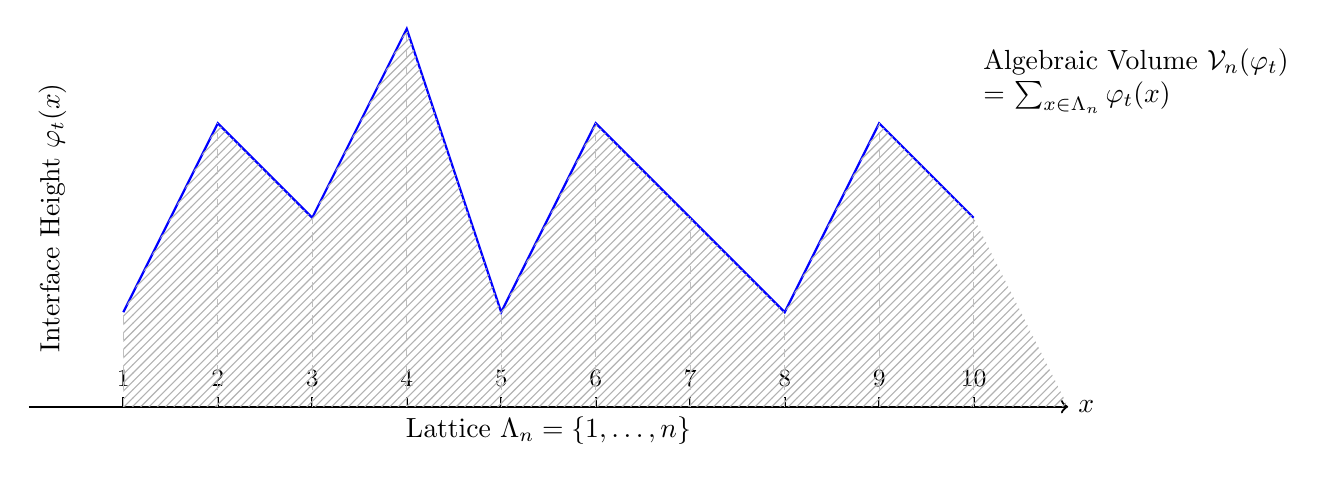
\begin{tikzpicture}[scale=1.2]
    % Define lattice parameters
    \def\n{10}   % Number of lattice sites
    \def\xmin{0} % Minimum x-coordinate
    \def\xmax{11} % Maximum x-coordinate (n+1 for better spacing)
    \def\ymax{4}  % Maximum y-coordinate for visualization
    
    % Define interface heights (sample configuration)
    \def\heights{{1,3,2,4,1,3,2,1,3,2}} % Heights at lattice sites 1 to 10
    
    % Draw x-axis
    \draw[thick, ->] (\xmin,0) -- (\xmax,0) node[right] {$x$};
    
    % Mark lattice sites on the x-axis
    \foreach \x in {1,...,\n} {
        \draw[thick] (\x,0) -- (\x,0.1) node[above] {\small \x};
    }
    
    % Draw fluctuating interface
    \draw[thick, blue] (1,\heights[0]) 
        \foreach \x in {2,...,\n} {
            -- (\x,\heights[\x-1])
        };
    
    % Fill the area under the interface (algebraic volume)
    \fill[pattern=north east lines, pattern color=gray!60] 
        (1,0) -- (1,\heights[0]) 
        \foreach \x in {2,...,\n} {
            -- (\x,\heights[\x-1])
        } -- (\xmax,0) -- cycle;
    
    % Draw vertical lines at lattice sites for better interface visualization
    \foreach \x in {1,...,\n} {
        \draw[dashed, gray!50] (\x,0) -- (\x,\heights[\x-1]);
    }
    
    % Add legend and labels
    \node at (0.5,\ymax/2) [rotate=90, above] {Interface Height $\varphi_t(x)$};
    \node[below] at (\xmax/2,0) {Lattice $\Lambda_n = \{1, \ldots, n\}$};
    \node[above right, align=left] at (\xmax-1,\ymax-1) {
        Algebraic Volume $\mathcal{V}_n(\varphi_t)$ \\ 
        = $\sum_{x \in \Lambda_n} \varphi_t(x)$
    };
\end{tikzpicture}
\end{document}